\section{Data Collection}
\label{sec:meth}

This section introduces \vt\ and 
discusses how we collect data from \vt\ and pre-process them.
We also present the analysis results of their basic properties, 
before delving into more advanced analysis in later sections.


\begin{table}[h!]
\centering
\footnotesize
{
\begin{tabular}{l|l}
\hline
Metadata Field & Explanation \\
\hline                            
%\cline{1-1}
{\bf name}      & submitted file name \\
{\bf link}      & where to download the file \\
{\bf timestamp} & timestamp when the submission was made \\
{\bf source\_country} & the country where the submission was made \\
{\bf source\_id} & user ID who made the submission\\
{\bf size} & file size \\
{\bf type} & file type \\
{\bf tags} & labels with more specific information for each {\bf type}\\
{\bf first\_seen} & when the same file was first submitted \\
{\bf last\_seen} & when the same file was last submitted \\
{\bf hashes} & sha1, sha256, md5, and vhash\\
{\bf ssdeep} & ssdeep digest string \\
{\bf total} & number of engines analyzing the file \\
{\bf positives} & number of engines that flagged the file as malicious \\
{\bf positives\_delta} & changes in {\bf positives} across different submissions\\
{\bf report} & detailed detection report from each AV engine \\
\hline
\end{tabular}
}
\caption{VirusTotal Metadata. 
%\footnotesize{
(Fields for each submission retrieved from VirusTotal through distribution API and their related explanation.
One file could be submitted multiple times by different users.)
%}
}
\label{tab:fields}
\end{table}



\subsection{VirusTotal}

\vt\ is a free online malware scan service.
It was founded in 2004 and was acquired by google in 2012. 
\vt\ is widely used by both normal users and anti-virus vendors.
Normal users submit suspicious files to \vt\ when they do not have any anti-virus software, 
or when they want to check for viruses possibly missed by their own anti-virus software 
or false alarms from their own anti-virus software.  
Anti-virus vendors use \vt\ to verify false positives and false negatives in their products~\cite{huangvt2016bigdata, neeles}.

For each submission, \vt\ applies a set of anti-virus engines to analyze it. 
\vt\ keeps information about whether the submission is labeled as malware by each engine, 
and detailed tags for identified malware from each engine. 

\vt\ provides open APIs to access and download both the metadata of all submissions and detection results.
One API, named distribution API, works like a pipe.
After a user opens the distribution API and starts to download data from \vt, 
\vt\ will keep returning metadata for latest submission to the user. 
%Roughly 20 GB data can be downloaded from \vt\ through distribution API.  

\vt\ provides rich metadata.
Table~\ref{tab:fields} shows the metadata fields and their meaning.  
The original submitted files from \vt\ can be downloaded using the {\bf link} field in the metadata.
{\color{red} TODO: discuss what metadata we use in Section 3 and Section 4}

\begin{figure}[t!]
\begin{center}
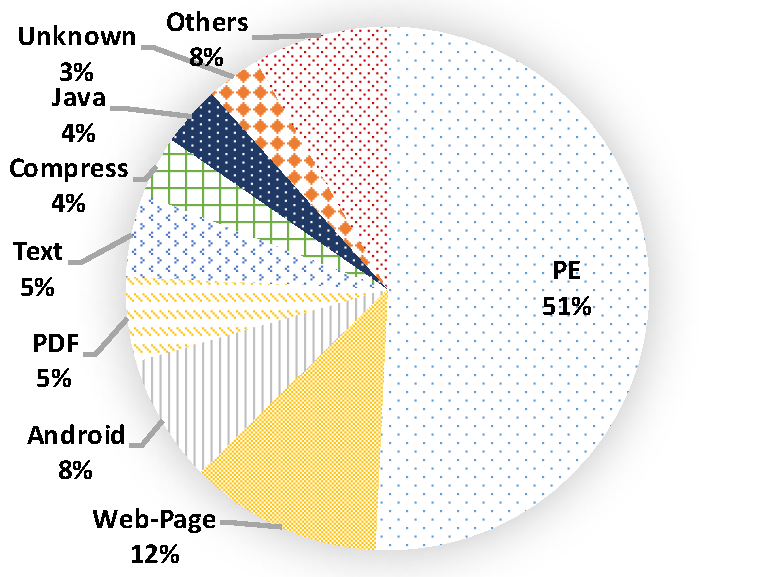
\includegraphics[width=2.in]{figure/type}
\caption{File type distributions.
%{\footnotesize{
(File types and their distributions for all VirusTotal submissions from 05/07/2016 to 09/06/2016.)
%}
}
\label{fig:type}
\end{center}
%\vspace{-0.25in}
\end{figure}


\subsection{Data Collection and Preprocessing}

We collected all metadata for all submissions to \vt\ from May 7th, 2016 to September 6th, 2016,
with a total of 151 million submissions. 
Our collected data is larger than or comparable to previous works on studying \vt~\cite{SongAPsys2016,huangvt2016bigdata}.
According to Lastline Labs~\cite{Lastline}, common lag time for an anti-virus engine to detect a new malware is two weeks.
Thus, four months' data is more than enough to analyze behaviors for most malware and anti-virus engines. 
Indeed, we drew several meaningful conclusions with this dataset, as will be presented in the rest of the paper.

We performed our data collection using \vt{}'s distribution API.
We insert all collected metadata into a table in Cassandra~\cite{cassandra} 
using the combination of sha256, source\_id, and timestamp as the key.
We then used Spark~\cite{spark} and wrote Spark programs to efficiently analyze the vast amount of data.
All our analysis is conducted by using Spark 1.4.0 on a cluster with 19 nodes, 266 cores, and 560 GB memory. 


Figure~\ref{fig:type} shows file type distributions for all submissions. 
Among all file types, Windows \textit{Portable Executable} ({\em \pe}) files, 
or ``Win32EXE'' and ``Win32DLL'' files, 
are the most frequently submitted type,
accounting for 51\% of all submissions.
Web pages and Android apps account for the second and third largest submissions, 
with 12\% and 8\% of all submissions respectively. 
Other popular file types include PDF, Text, compressed files, and Java files. 
This result shows that even though new types of malware such as Android apps have
increased significantly in recent years, 
traditional types of malwares such as \pe\ files and web pages are still the 
most commonly targeted by attackers.

Since PE files are the most common type,
we focus our study in this paper on \pe\ files 
and leave studies on other types of malwares for future. 
%If the type field for a submission is either ``Win32EXE'' or ``Win32DLL'', 
%we consider the submission is a PE file. 
In total, we collected 76 million \pe\ submissions.


\subsection{Caveats}
Like all other empirical studies, 
our findings and conclusions need to be considered with our methodology in mind. 
We use the distribution API provided by \vt\ to download submissions' metadata 
from \vt. 
There is no guarantee that this API returns all submissions to \vt.
%all data can be successfully downloaded. 
It could be possible that some files are submitted to \vt, 
but are not downloaded. %we fail to get their information from \vt.
Although we have collected huge amount of malware information from \vt,
we do believe that there are malware never submitted to \vt, 
or submitted to \vt much later than when they appear in the real world. 
However, there are no conceivable ways to study them.
We believe that the 4-month malware information we collect can serve as a representative sample for malware in the real world. 